%% Basierend auf einer TeXnicCenter-Vorlage von Mark Müller
%%%%%%%%%%%%%%%%%%%%%%%%%%%%%%%%%%%%%%%%%%%%%%%%%%%%%%%%%%%%%%%%%%%%%%%

% Wählen Sie die Optionen aus, indem Sie % vor der Option entfernen  
% Dokumentation des KOMA-Script-Packets: scrguide

%%%%%%%%%%%%%%%%%%%%%%%%%%%%%%%%%%%%%%%%%%%%%%%%%%%%%%%%%%%%%%%%%%%%%%%
%% Optionen zum Layout des Artikels                                  %%
%%%%%%%%%%%%%%%%%%%%%%%%%%%%%%%%%%%%%%%%%%%%%%%%%%%%%%%%%%%%%%%%%%%%%%%
\documentclass[%
%a5paper,							% alle weiteren Papierformat einstellbar
%landscape,						% Querformat
%10pt,								% Schriftgröße (12pt, 11pt (Standard))
%BCOR1cm,							% Bindekorrektur, bspw. 1 cm
%DIVcalc,							% führt die Satzspiegelberechnung neu aus
%											  s. scrguide 2.4
%twoside,							% Doppelseiten
%twocolumn,						% zweispaltiger Satz
%halfparskip*,				% Absatzformatierung s. scrguide 3.1
%headsepline,					% Trennline zum Seitenkopf	
%footsepline,					% Trennline zum Seitenfuß
%titlepage,						% Titelei auf eigener Seite
%normalheadings,			% Überschriften etwas kleiner (smallheadings)
%idxtotoc,						% Index im Inhaltsverzeichnis
%liststotoc,					% Abb.- und Tab.verzeichnis im Inhalt
%bibtotoc,						% Literaturverzeichnis im Inhalt
%abstracton,					% Überschrift über der Zusammenfassung an	
%leqno,   						% Nummerierung von Gleichungen links
%fleqn,								% Ausgabe von Gleichungen linksbündig
%draft								% überlangen Zeilen in Ausgabe gekennzeichnet
]
{scrartcl}

%\pagestyle{empty}		% keine Kopf und Fußzeile (k. Seitenzahl)
%\pagestyle{headings}	% lebender Kolumnentitel

%% Deutsche Anpassungen %%%%%%%%%%%%%%%%%%%%%%%%%%%%%%%%%%%%%
\usepackage[english]{babel}
\usepackage[T1]{fontenc}
\usepackage[utf8]{inputenc}

\usepackage{amsthm} % Theorem-Packet
\usepackage{amsmath}
\usepackage{amssymb}

\usepackage{stmaryrd} % Blitzsymbol
\usepackage{fancyhdr} % Für Kopfzeile
\usepackage{graphicx} % Einbinden von Grafiken
\usepackage{bbding} % Für das Häckchen
\usepackage{amscd} % Kommutative Diagramme
\usepackage{mathtools} % Für das Definitionssymbol

\usepackage{listings}
\usepackage{courier}

\pagestyle{fancy}
\lhead{QGD411}\chead{Exercise notes: Driven Pendulum - Cyclotrons - Black Holes}\rhead{HS 2013} % Kopfzeile

\newtheoremstyle{plain}%  name
  {.5\baselineskip}% Space above
  {.5\baselineskip}% Space below
  {}% Body font
  {}% Indent amount (empty = no indent, \parindent = para indent)
  {\bfseries}% Thm head font
  {:}% Punctuation after thm head
  { }% Space after thm head: " " = normal interword space; \newline = linebreak
  {}% Thm head spec (can be left empty, meaning `normal')
  
\makeatletter % Matrizen mit opitonalen Linien
\renewcommand*\env@matrix[1][*\c@MaxMatrixCols c]{%
  \hskip -\arraycolsep
  \let\@ifnextchar\new@ifnextchar
  \array{#1}}
\makeatother

\theoremstyle{plain}
\newtheorem*{bsp}{Beispiel} % Beispiele ohne Nummerierung
\newtheorem*{bws}{Beweis} % Beweise ohne Nummerierung 
\newenvironment{beweis}{\begin{bws}~\vspace{0.5\baselineskip}}{\hfill $\qedsymbol$\end{bws}}
\newenvironment{beispiel}{\begin{bsp}~\vspace{0.5\baselineskip}}{\end{bsp}}

\usepackage{lmodern} % Type1-Schriftart für nicht-englische Texte

\usepackage{enumerate}

\renewcommand\theenumi{\roman{enumi}}
\renewcommand\labelenumi{\theenumi)}

%% Packages für Grafiken & Abbildungen %%%%%%%%%%%%%%%%%%%%%%
%\usepackage{graphicx} %%Zum Laden von Grafiken
%\usepackage{subfig} %%Teilabbildungen in einer Abbildung
%\usepackage{tikz} %%Vektorgrafiken aus LaTeX heraus erstellen

%\setlength{\parindent}{0pt} % kein Einzug


%% Beachten Sie:
%% Die Einbindung einer Grafik erfolgt mit \includegraphics{Dateiname}
%% bzw. über den Dialog im Einfügen-Menü.
%% 
%% Im Modus "LaTeX => PDF" können Sie u.a. folgende Grafikformate verwenden:
%%   .jpg  .png  .pdf  .mps
%% 
%% In den Modi "LaTeX => DVI", "LaTeX => PS" und "LaTeX => PS => PDF"
%% können Sie u.a. folgende Grafikformate verwenden:
%%   .eps  .ps  .bmp  .pict  .pntg


%% Bibliographiestil %%%%%%%%%%%%%%%%%%%%%%%%%%%%%%%%%%%%%%%%%%%%%%%%%%
%\usepackage{natbib}

\begin{document}

\lstset{basicstyle=\ttfamily, breakatwhitespace=false, breaklines=true, frame=single, xleftmargin=\parindent, aboveskip=\baselineskip, belowskip=\baselineskip}

%\pagestyle{empty} %%Keine Kopf-/Fusszeilen auf den ersten Seiten.


%%%%%%%%%%%%%%%%%%%%%%%%%%%%%%%%%%%%%%%%%%%%%%%%%%%%%%%%%%%%%%%%%%%%%%%
%% Ihr Artikel                                                       %%
%%%%%%%%%%%%%%%%%%%%%%%%%%%%%%%%%%%%%%%%%%%%%%%%%%%%%%%%%%%%%%%%%%%%%%%

%% eigene Titelseitengestaltung %%%%%%%%%%%%%%%%%%%%%%%%%%%%%%%%%%%%%%%    
%\begin{titlepage}
%Einsetzen der TXC Vorlage "Deckblatt" möglich
%\end{titlepage}

%% Angaben zur Standardformatierung des Titels %%%%%%%%%%%%%%%%%%%%%%%%
\titlehead{\center{University of Zurich - HS 2013}}
%\subject{Typisierung}
\title{Computational Science I\\Exercise notes: Driven Pendulum - Cyclotrons - Black Holes\\\rule{1.0\textwidth}{1.0pt}}
\author{Tobias Grubenmann}
%\and{Der Name des Co-Autoren}
%\thanks{Fußnote}			% entspr. \footnote im Fließtext
%\date{}							% falls anderes, als das aktuelle gewünscht
%\publishers{Herausgeber}

%% Widmungsseite %%%%%%%%%%%%%%%%%%%%%%%%%%%%%%%%%%%%%%%%%%%%%%%%%%%%%%
%\dedication{Widmung}

\maketitle 						% Titelei wird erzeugt

%% Zusammenfassung nach Titel, vor Inhaltsverzeichnis %%%%%%%%%%%%%%%%%
%\begin{abstract}
% Für eine kurze Zusammenfassung des folgenden Artikels.
% Für die Überschrift s. \documentclass[abstracton].
%\end{abstract}

%% Erzeugung von Verzeichnissen %%%%%%%%%%%%%%%%%%%%%%%%%%%%%%%%%%%%%%%
%\tableofcontents			% Inhaltsverzeichnis
%\listoftables				% Tabellenverzeichnis
%\listoffigures				% Abbildungsverzeichnis


%% Der Text %%%%%%%%%%%%%%%%%%%%%%%%%%%%%%%%%%%%%%%%%%%%%%%%%%%%%%%%%%%

\section*{Exercise 1}

The following code solves the problem of the driven pendulum with the built-in ODE solver from Python:

\lstinputlisting[language=Python]{../drivenPendulumODEInt.py}

The first picture shows the surface of section for intial $p$ between 0 and 1 with $\omega = -2$ and $\varepsilon = 0.3$. The simulation ran until $\omega t=40\pi$.

\begin{center}
\centering
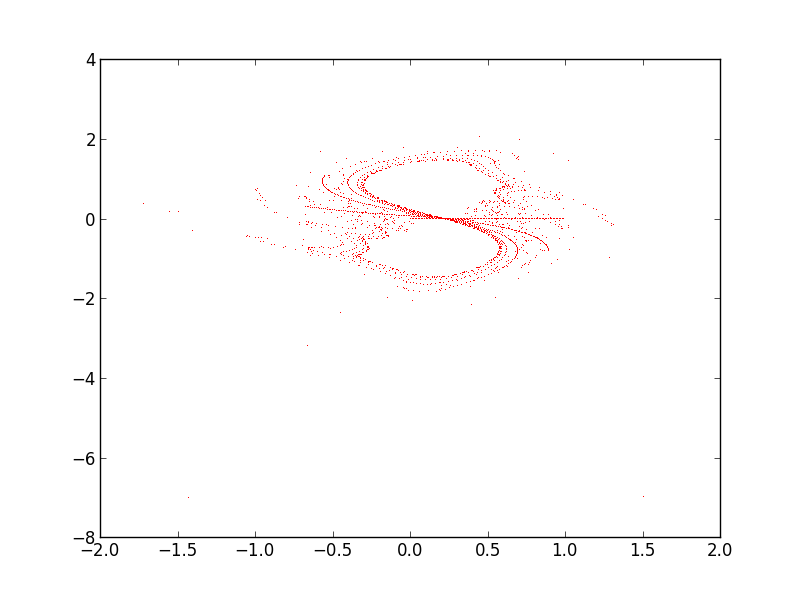
\includegraphics[width=0.6\linewidth]{../drivenPendulumODEInt.png}
\captionof{figure}{Driven pendulum for different intitial $p$ between 0 and 1, until $\omega t=40\pi$ with the Python solver}
\end{center}

The second picture shows the same as the first but the simulation ran until $\omega t=200\pi$.

\begin{center}
\centering
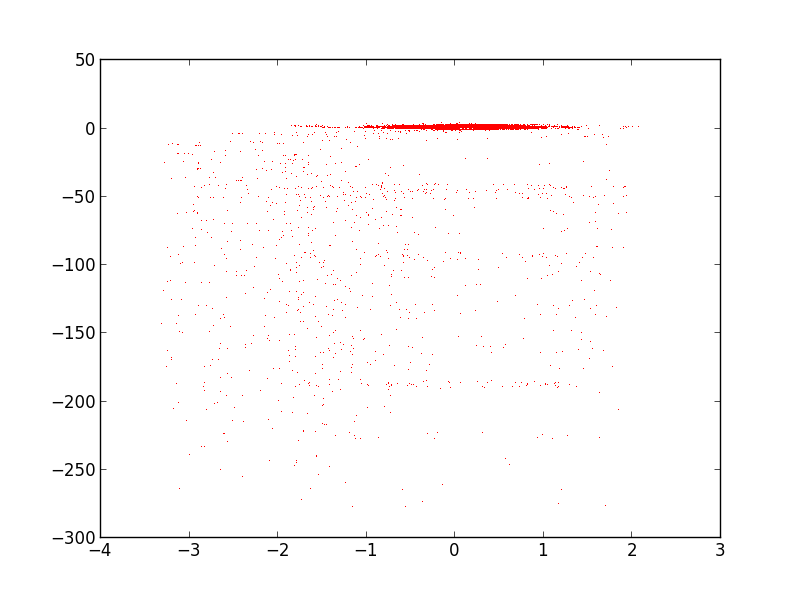
\includegraphics[width=0.6\linewidth]{../drivenPendulumODEInt2.png}
\captionof{figure}{Driven pendulum for different intitial $p$ between 0 and 1, until $\omega t=200\pi$ with the Python solver}
\end{center}

The following code solves the problem of the driven pendulum with the Leapfrog method:

\lstinputlisting[language=Python]{../drivenPendulumLeapfrog.py}

The first picture shows the surface of section for intial $p$ between 0 and 1 with $\omega = -2$ and $\varepsilon = 0.3$. The simulation ran until $\omega t=40\pi$.

\begin{center}
\centering
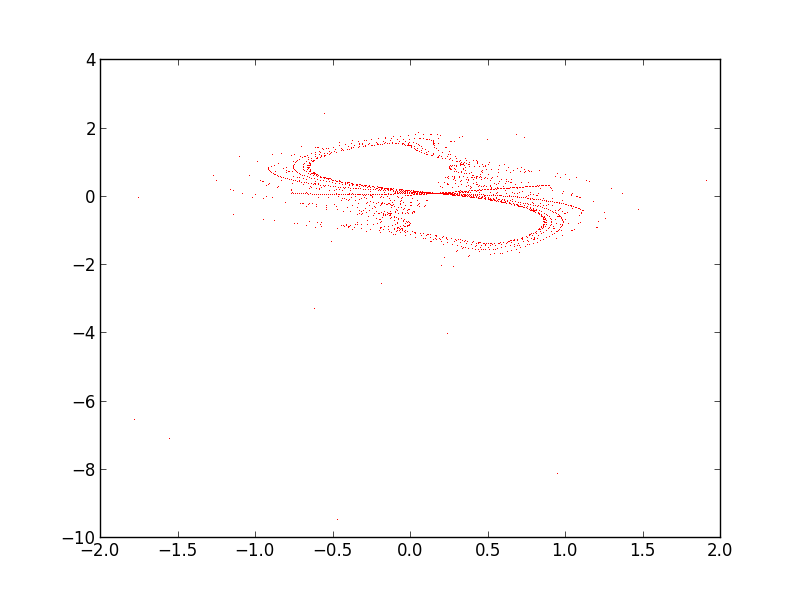
\includegraphics[width=0.6\linewidth]{../drivenPendulumLeapfrog.png}
\captionof{figure}{Driven pendulum for different intitial $p$ between 0 and 1, until $\omega t=40\pi$ with the Leapfrog solver}
\end{center}

The second picture shows the same as the first but the simulation ran until $\omega t=200\pi$.

\begin{center}
\centering
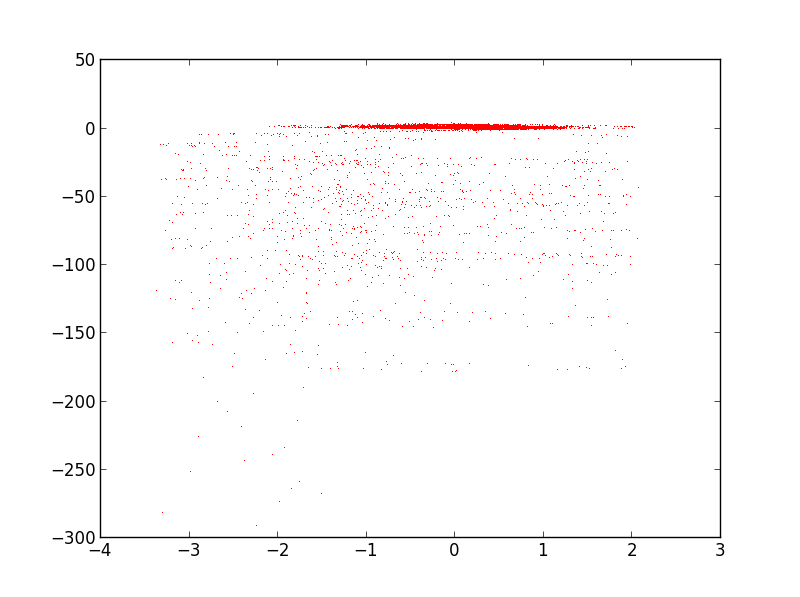
\includegraphics[width=0.6\linewidth]{../drivenPendulumLeapfrog2.png}
\captionof{figure}{Driven pendulum for different intitial $p$ between 0 and 1, until $\omega t=200\pi$ with the Leapfrog solver}
\end{center}

\section*{Exercise 2}

To solve the cyclotron problem we need first to get the differential equations from the Hamiltonian. For the relativistic case this gives the following system:

\begin{eqnarray*}
\dot{x}&=&\frac{p_{x}+y}{\sqrt{1+(p_{x}+y)^{2}+(p_{y}-x)^{2}}}\\
\dot{y}&=&\frac{p_{y}-x}{\sqrt{1+(p_{x}+y)^{2}+(p_{y}-x)^{2}}}\\
\dot{p_{x}}&=&\frac{p_{y}-x}{\sqrt{1+(p_{x}+y)^{2}+(p_{y}-x)^{2}}}\\
\dot{p_{x}}&=&-\frac{p_{x}+y}{\sqrt{1+(p_{x}+y)^{2}+(p_{y}-x)^{2}}}+\alpha\cos(\omega t)
\end{eqnarray*}\\

For the non-relativistic case we have the following system:

\begin{eqnarray*}
\dot{x}&=&p_{x}+y\\
\dot{y}&=&p_{y}-x\\
\dot{p_{x}}&=&p_{y}-x\\
\dot{p_{x}}&=&-p_{x}-y+\cos(\omega t)
\end{eqnarray*}\\

The following code solves for the relativistic case:

\lstinputlisting[language=Python]{../cyclotronsRelativistic.py}

The following pictures shows the plots of $x,y,p_{x},p_{y}$ for the relativistic case for different $\omega$ and $\alpha$:

\begin{center}
\centering
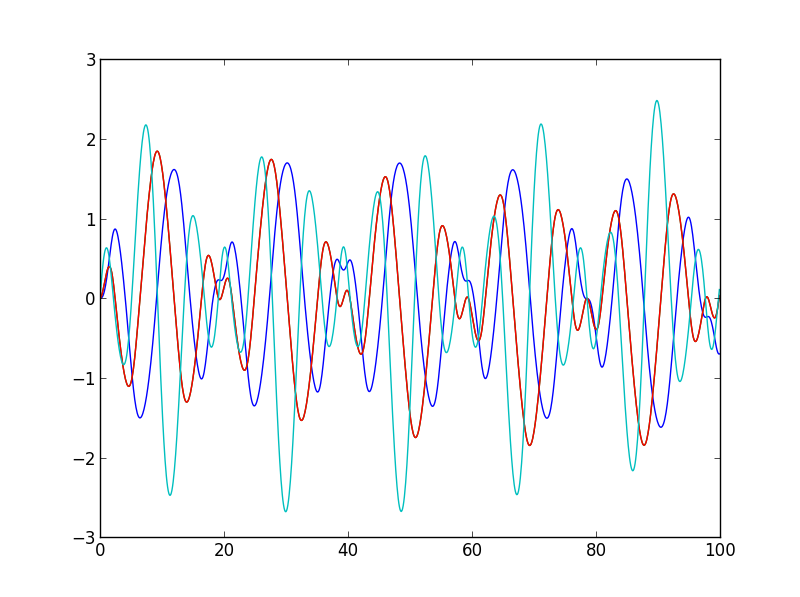
\includegraphics[width=0.6\linewidth]{../cyclotronsRelativistic_o1_a1.png}
\captionof{figure}{$x,y,p_{x},p_{y}$ for a cyclotron with $\omega=1$, $\alpha=1$}
\end{center}

\begin{center}
\centering
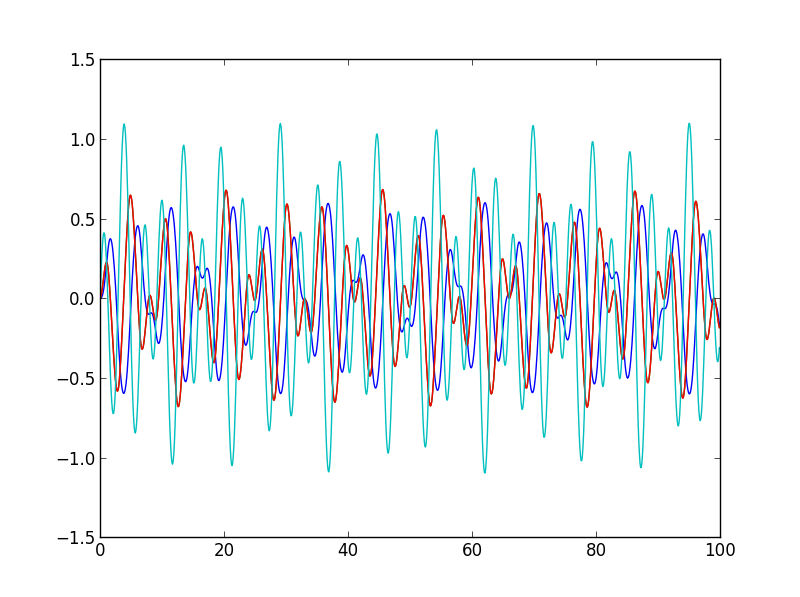
\includegraphics[width=0.6\linewidth]{../cyclotronsRelativistic_o2_a1.png}
\captionof{figure}{$x,y,p_{x},p_{y}$ for a cyclotron with $\omega=2$, $\alpha=1$}
\end{center}

\begin{center}
\centering
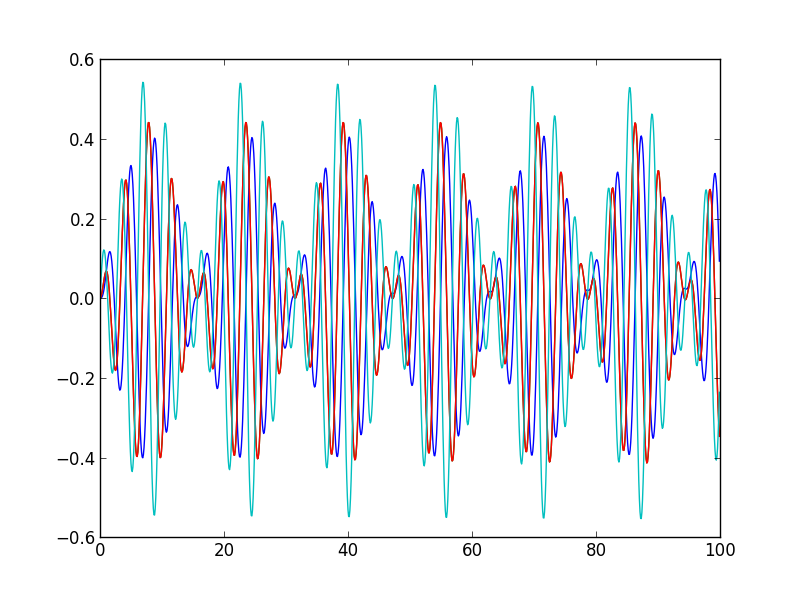
\includegraphics[width=0.6\linewidth]{../cyclotronsRelativistic_o2_a03.png}
\captionof{figure}{$x,y,p_{x},p_{y}$ for a cyclotron with $\omega=2$, $\alpha=0.3$}
\end{center}

\begin{center}
\centering
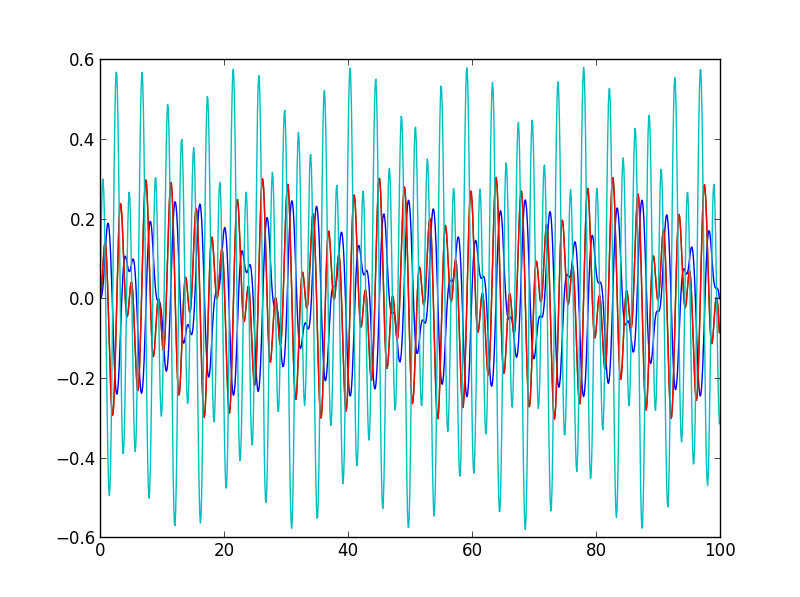
\includegraphics[width=0.6\linewidth]{../cyclotronsRelativistic_o3_a1.png}
\captionof{figure}{$x,y,p_{x},p_{y}$ for a cyclotron with $\omega=3$, $\alpha=1$}
\end{center}

The following code solves for the non-relativistic case:

\lstinputlisting[language=Python]{../cyclotronsNonRelativistic.py}

The following pictures shows the plots of $x,y,p_{x},p_{y}$ for the non-relativistic case for different $\omega$:

\begin{center}
\centering
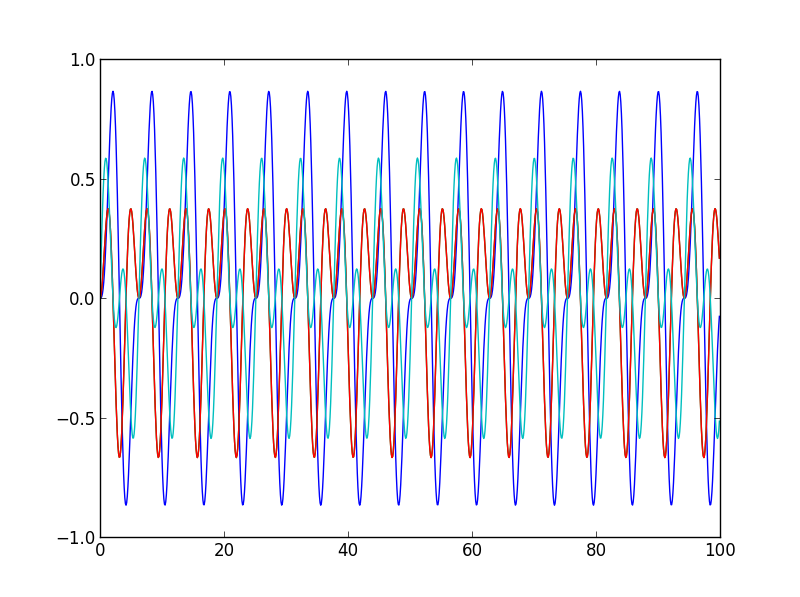
\includegraphics[width=0.6\linewidth]{../cyclotronsNonRelativistic_o1.png}
\captionof{figure}{$x,y,p_{x},p_{y}$ for a cyclotron with $\omega=1$}
\end{center}

\begin{center}
\centering
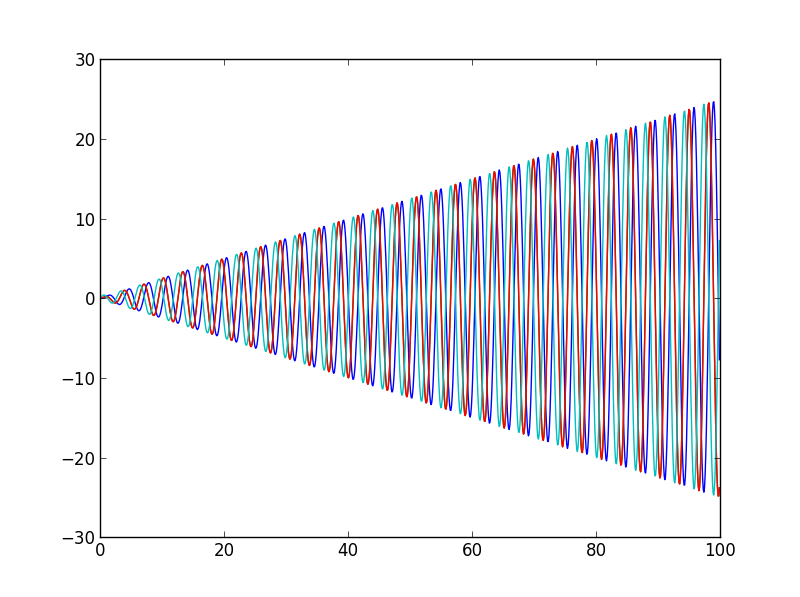
\includegraphics[width=0.6\linewidth]{../cyclotronsNonRelativistic_o2.png}
\captionof{figure}{$x,y,p_{x},p_{y}$ for a cyclotron with $\omega=2$}
\end{center}

\begin{center}
\centering
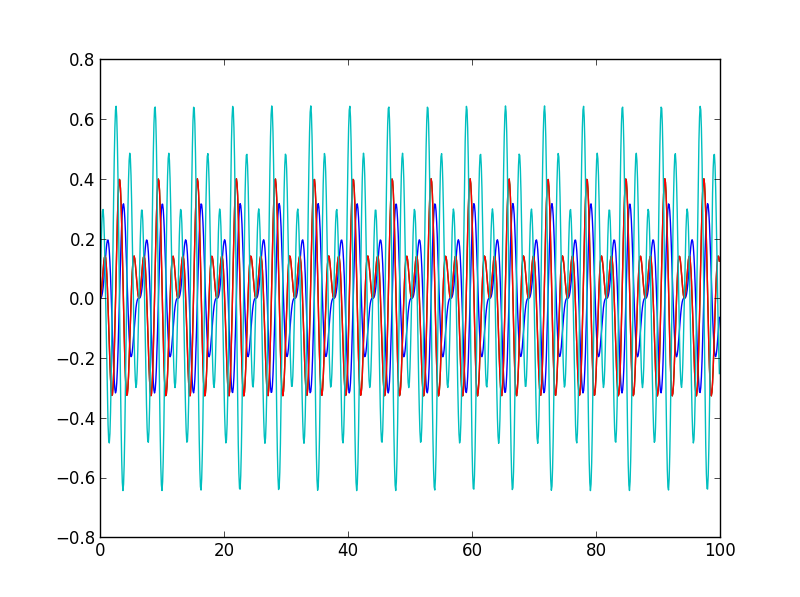
\includegraphics[width=0.6\linewidth]{../cyclotronsNonRelativistic_o3.png}
\captionof{figure}{$x,y,p_{x},p_{y}$ for a cyclotron with $\omega=3$}
\end{center}

\section*{Exercise 3}

To solve this problem we need first to get the differential equations from the Hamiltonian:

\begin{eqnarray*}
\dot{x}&=&p_{x}-\frac{2(xp_{x}+yp_{y})x}{r^{3}}\\
\dot{y}&=&p_{y}-\frac{2(xp_{x}+yp_{y})y}{r^{3}}\\
\dot{p_{x}}&=&-\frac{1}{2}\left(1-\frac{2}{r}\right)^{-2}\frac{2}{r^{2}}\cdot\frac{x}{r}+\frac{2(xp_{x}+yp_{y})p_{x}\cdot r^{3}-(xp_{x}+yp_{y})^{2}3r^{2}\cdot\frac{x}{r}}{r^{6}}\\
\dot{p_{x}}&=&-\frac{1}{2}\left(1-\frac{2}{r}\right)^{-2}\frac{2}{r^{2}}\cdot\frac{y}{r}+\frac{2(xp_{x}+yp_{y})p_{y}\cdot r^{3}-(xp_{x}+yp_{y})^{2}3r^{2}\cdot\frac{y}{r}}{r^{6}}
\end{eqnarray*}\\

The following code solves the black hole problem:

\lstinputlisting[language=Python]{../blackHole.py}

The following figures show the orbit for an initial velocity of $(0, 0.2)$ and different initial positions:

\begin{center}
\centering
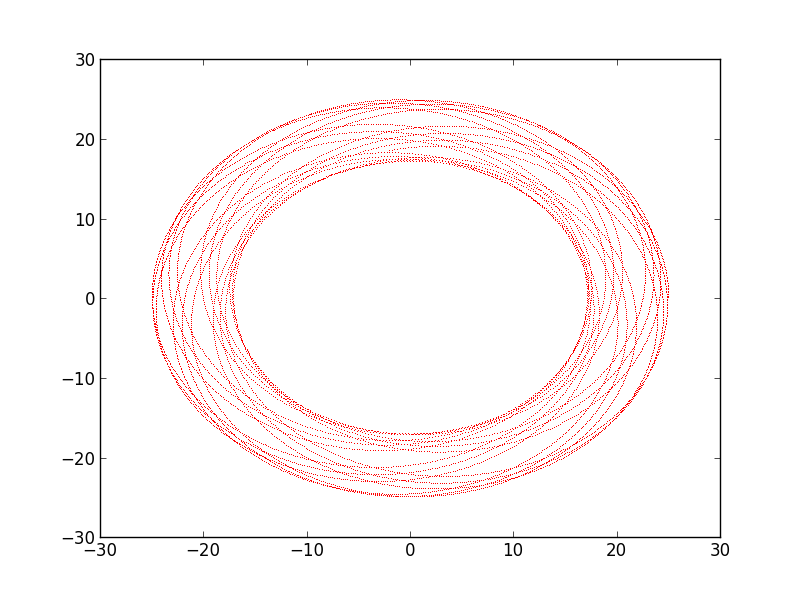
\includegraphics[width=0.6\linewidth]{../blackHole25.png}
\captionof{figure}{Orbit near a black hole with initial position $(25, 0)$}
\end{center}

\begin{center}
\centering
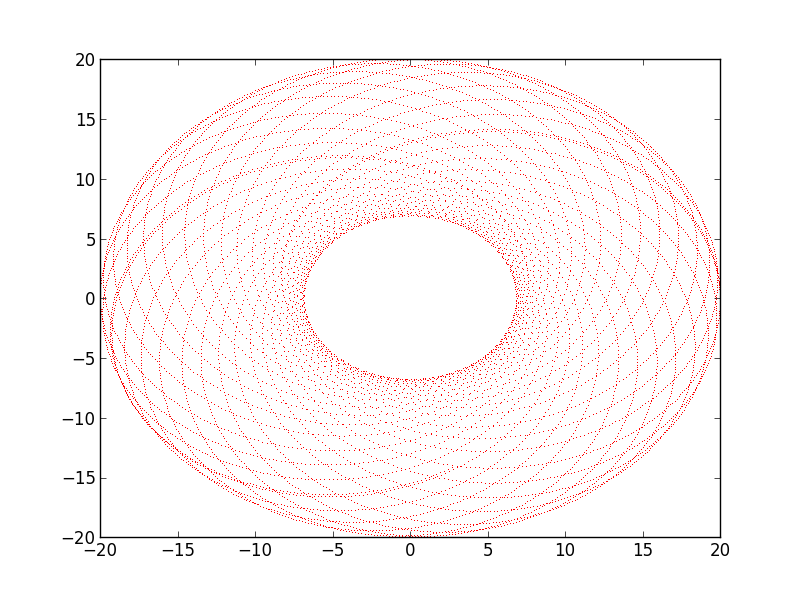
\includegraphics[width=0.6\linewidth]{../blackHole20.png}
\captionof{figure}{Orbit near a black hole with initial position $(20, 0)$}
\end{center}

\begin{center}
\centering
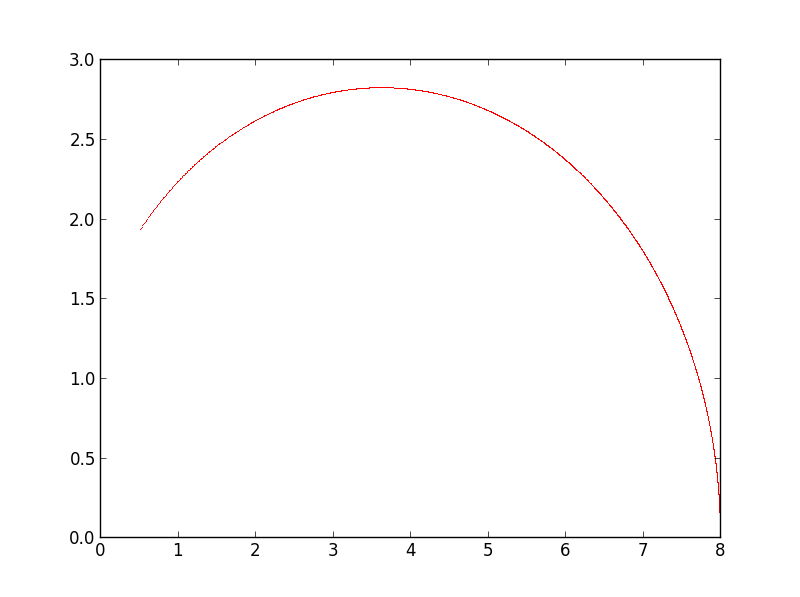
\includegraphics[width=0.6\linewidth]{../blackHole8.png}
\captionof{figure}{Orbit near a black hole with initial position $(8, 0)$}
\end{center}

%% Bibliographie unter Verwendung von dinnat %%%%%%%%%%%%%%%%%%%%%%%%%%
%\setbibpreamble{Präambel}		% Text vor dem Verzeichnis
%\bibliographystyle{dinat}
%\bibliography{bibliographie}	% Sie benötigen einen *.bib-Datei

\end{document}




